\documentclass[12pt]{article}
\usepackage{graphicx}
\usepackage{enumerate}
\usepackage{booktabs}
\usepackage{amsmath}
\usepackage[T1]{fontenc}
\author{Aaron Song s267807}
\title{CW2}
\date{\today}


\begin{document}
\maketitle



\section{Task 1}

1. An entry of data in this problem is defined as $(x,y,label)$, where $x$ and $y$ is the inputs and $label$ is the output. Define:
\begin{description}
    \item[data] Data: x:number, y:number, label: number
    \item[neural network] A neural network in this task is an object with a function that takes a pair of numbers of outputs a number, so functionally define Apply: number->number->number and NeuralNetwork: { Apply } (an object with an Apply function).
    \item[loss function] Loss can be defined as:
    \begin{gather*}
    \textrm{Loss(nn: NeuralNetwork, d: Data)} = ((\textrm{Apply d.x d.y)-d.error)}^2
    \end{gather*}
    \item[fitness functtion] The fitness of a neural network is the average loss on the specific dataset. 
    \begin{gather*}
    \textrm{Ftiness(nn: NeuralNetwork, ds: Data[])} = \frac{\sum_{i=1}^{\textrm{ds.Length}}Loss(nn, ds[i])}{ds.Length}
    \end{gather*}
\end{description}

\noindent 2. A [-10, 10] is enough for this question.

\noindent 3. Two hidden layers are used, with the first 5~7 neurons and the second 2 neurons. If only one hidden layer is permitted, 7 neurons are prefered to get a better result, as shown in Figure \ref{7n}.\\
With PSO, as shown in Figure \ref{pso_7n}, the best result achieved is the test loss of 0.119. The performance is much worser than stochastic gradient descent.
\begin{figure}[!ht]
\centering
\begin{minipage}[t]{0.48\textwidth}
    \centering
    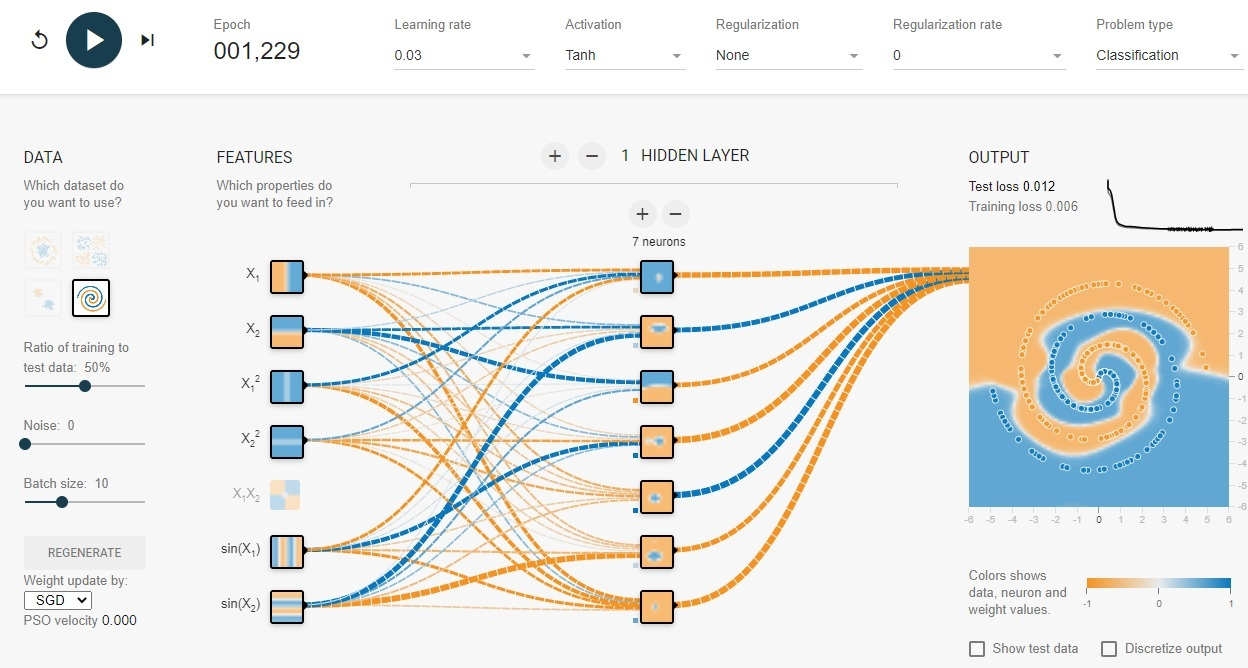
\includegraphics[width=\textwidth]{1.jpg}
    \caption{A hidden layer with 7 neurons}
    \label{7n}
\end{minipage}
\begin{minipage}[t]{0.48\textwidth}
    \centering
    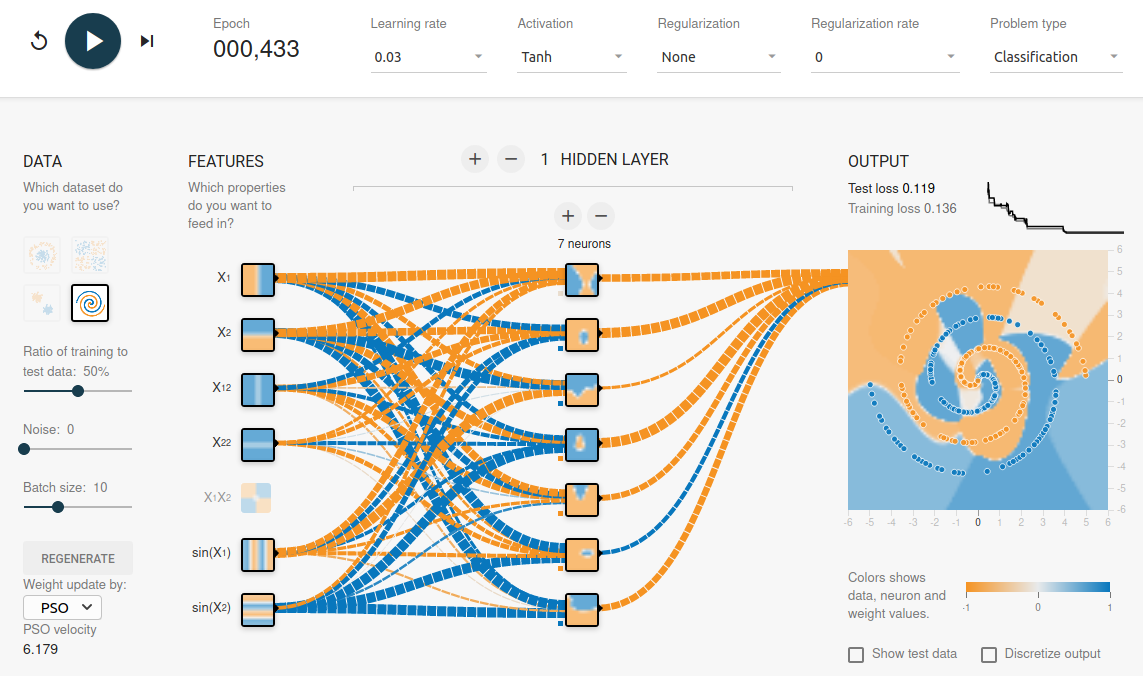
\includegraphics[width=\textwidth]{PSO.png}
    \caption{Using PSO to optimize weights}
    \label{pso_7n}
\end{minipage}
\end{figure}


\noindent 4.
The learning result is much better when non-linear input are involved. For this question specifically, a spiral data is generated by a formula $r=k\theta$ where $k>0, \theta>0$. When translating the polar coordinate into a Cartisean coordinate, it's 
\begin{equation}
\label{equ:task1-target-func}
\sqrt{x^2+y^2}=k(2n\pi+\textrm{atan2}(x,y))
\end{equation}
, where $n\in Z$ and atan2 is the arctan function defined by most common programming language where the range is $[0,2\pi)$. In order to expand the aforementioned equation into a plain form, atan2 can be approximately translated into $\arctan$, and according to Tylor expansion, 
\begin{gather*}
\frac{\textrm{d}\arctan x}{\textrm{d}x}=\frac{1}{x+1}\\
\arctan x=x-\frac{1}{3}x^3+\frac{1}{5}x^5-\ldots
\end{gather*}
. Curtailling high order terms, 
\begin{gather*}
\arctan x=x-\frac{1}{3}x^3\\
x^2+y^2=an+b(x-\frac{1}{3}x^3)^2
\end{gather*}
where $a=\frac{4k^2}{\pi^2},b=k^2$. Curtailling high order terms again, 
\begin{gather*}
x^2+y^2=an+bx
\end{gather*}
We can see that $x^2$, $y^2$, terms are presented here. To fully simulate the spiral data generation function \ref{equ:task1-target-func}, $\sin x$ and $\sin y$ may also be included given the Tylor expansion:
\begin{gather*}
\sin x=x-\frac{1}{3!}x^3+\frac{1}{5!}x^5-\ldots
\end{gather*}

Therefore theoratically, an architecture with only linear input features performs worse than one with non-linear features. Practically, it's very hard for us to find a set of parameters to keep the test loss under 0.2 for a purely linear-feature architecture.

\noindent 5. Many NN parameters have an effect to this particular problem.

\noindent \textbf{learning rate} The learning rate decides how fast the weights and biases of the neural network changes. A moderate value (0.03 or 0.1) yields good output, otherwise if it's too high ($\geq 1$) the training loss and the test lost will fluctuate too fast and fail to converge to a proper local best. If too small ($\leq 0.0003$), the weights and the biases barely change. A global best may still present itself after enough long time, but that may take too many epochs.

\noindent \textbf{activation function} Activation function is used to determine whether a neuron is activated (that means if it yields a result of not). It's also used to normalise the output of a neuron to a range [-1, 1] so that every neuron has a relatively equal impact on the result of a layer of the nn. 
\begin{itemize}
\item \textbf{linear} The linear function is bad to be used as the AF because they fail to normalise the output of a neuron. Also, since a linear combination of linear functions is also a linear function and each layer of the NN is a linear combination of the last layer, using linear as AF in an NN consequently set the number of layer of the NN to 1.
\item \textbf{Sigmoid} or \textbf{Tanh} Sigmoid and Tanh are quite similar in that they are both able to smmoth and normalise the output. In case that they are computationally expensive, we can utilise the Tylor expansion at $x=0$ and expends the function to $x^5$ to simulate.
\item \textbf{ReLU} ReLU is not applicable as well because this problem includes negative values. A modified ReLU may be more useful, such as leaky ReLU (for example, $y=\max(0.1\times x, x)$).
\end{itemize}

\noindent \textbf{regularisation} Regularisation means a penalty for large weights by adding an additional term that is affected by the weight of each neuron. It is usually utilised to prevent overfitting on given data. Now with regularisation, the loss function would be:
\begin{gather*}
\widehat{Y}=\sum_1^n\omega_i x_i+b\\
\textrm{Loss}=Error(Y, \widehat{Y})+\lambda\sum_1^n r(\omega_i)
\end{gather*}
, where $\lambda$ is the regularisation rate and $r(x)$ is the regularisation function. Typically, L1 regularisation means $r(x)=|x|$ and L2 regularisation means $r(x)=x^2$.
Normally the correct usage of the regularisation facilitates a better result, but in this assignment neither L1 nor L2 regularisation refines the result a bit. It's only noticing when the regularisation rate is too big (higher than 0.003) the weights of many nodes drop to 0 quickly and never rebounce, causing these nodes dead.

\noindent \textbf{feature} The features in this problem are the only source of non-linear input and decide the form of the neural network; the number of layers and the number of neurons on each layer depend only the linear combination of the input features. As memtioned in the previous question, $x_1^2$ and $\sin x$ improve the learning result a lot compared to a purely linear model. I also tried $x_1^3$ and $x_2^3$, but the result is not satisfying.

\noindent \textbf{nn shape} Every neural node blends all inputs linearly and yields one single value. Mathematically, suppose there are $x$ layers (including the input layer) of nodes in the neural network and on layer $i$ there are $k[i]$ nodes ($0\leq i<x$), then node $b$ on layer $0<a\leq x$ $n_{a,b}$ takes a vector 
$X=(x_0,x_1,\ldots,x_{k[a-1]})$ as input and output $A\cdot X+B$, where $A$ stands for the weight between $a-1$ layer and node $n_{a,b}$ and $B$ represents the bias of node $n_{a,b}$.\\
In other words, the input layer is defined by some common function $y=x$, $y=x^2$, $y=\sin x$, and nodes in a following layers form a linear combination of the last layer.
    
      
\begin{description}
\item[Inertia weight $\omega$]  $\omega$ is the weight that is given to the previous velocity. Tuning $\omega$ will affect the balance between exploitation and exploration. If $\omega = 0$, particles will only move toward personal best and global best. If $\omega > 0$, the particles will have some exploitation of local space. \\
There is an experiment of different $\omega$ choice on a NN with 1 hidden layer, input features [$x_1,x_2,x_1^2,x_2^2,\sin(x_1),\sin(x_2)$], learning rate = 0.03, activation = Tanh, no regularization. $\alpha_1=\alpha_2 = 1.5$, swarm size = 100.
Results shown in Table \ref{t_omega}.
\begin{table}[!ht]
\centering
\begin{tabular}{@{}cccc@{}}
\toprule
$\omega$ & Average Test Loss & Epoches before stable \\ \midrule
0 & 0.43 & 50  \\
0.5 & 0.33  &  100  \\
0.7 & 0.22  &   400 \\
1  & 0.48  & Not Stable  \\
\bottomrule
\end{tabular}
\caption{Performance with different $\omega$}
\label{t_omega}
\end{table}
\\
The higher $\omega$, the more epoches are required to converge. If $\omega = 1$, the particles will keep on flying with increasing volocity.\\
Due to the stochastic of PSO, the test loss is not same at each run. 
\end{description}
\begin{description}
\item[accelerate constant $\alpha_1$ and $\alpha_2$ ] 

$\alpha_1$ and $\alpha_2$ describe the acceleration toward personal best and global best of a particle.
Small acceleration may cause the particles to fly around the goal area, and large acceleration may result in particle moving fast to the goal or even pass away from goal. If $\alpha_1 = 0$, the particle has no self-awareness, and will always get to new search space. It may converge faster, but it could lead to local minima. If $\alpha_2=0$, there is no interaction among particles, the particles will move alone. It probably won't converge.
Typically, $\alpha_1 = \alpha_2$.

\begin{table}[!ht]
\centering
\begin{tabular}{@{}cccc@{}}
\toprule
$\alpha_1$,$\alpha_2$ & Average Test Loss & PSO velocity \\ \midrule
1 & 0.36 & 3 to 5  \\
1.5 & 0.22  &  6 to 10  \\
2 & 0.39  &   7 to 12 \\
5  & 0.48  &  40 to 50  \\
\bottomrule
\end{tabular}
\caption{Performance with different $\alpha$}
\label{t_alpha}
\end{table}
The higher $\alpha$, the higher velocity of PSO.
If $\alpha_1 = 0$, the velocity reaches to 0 rapidly, but the test loss is above 0.5. If $\alpha_2 = 0$, the velocity does not reach to 0, but it is also worse than a random algorithm.

\end{description}
\begin{description}
\item[swarm size]
Swarm size is the number of particles. Larger swarm size could improve accuracy in difficult problems. Swarm size can critically affect the iteration time of an epoch.
\begin{table}[!ht]
\centering
\begin{tabular}{@{}cccc@{}}
\toprule
Swarm Size & Average Test Loss  \\ \midrule
10 & 0.32 \\
30 & 0.32    \\
100 & 0.22  \\
1000  & 0.22   \\
\bottomrule
\end{tabular}
\caption{Performance with different swarm size}
\label{t_swarm}
\end{table}
\end{description}

\begin{description}
\item[minimum and maximum velocity]
This is not implemented in the Playground, but it might have some influence. If the velocity is large, the particle may skip an optimum solution. If it is too small, the particle may get stuck with local minima.
\end{description}

\section{Task 2}
There're seven input nodes so the encoding of the input layer would be a binary string with a length of 7; the maximum number of layers is 6 and on each layer the limit of the number of neurons is 8, so a layer can be encoded in a binary string with a length of 3. In the first layer (also the input layer), every node is different because each one represents a different input function (it is however possible to have to input nodes with the same function, but it would be meaningless); for other layers, every node (neuron) is the same. So the neural network can be represented as:
$$
{i_0i_1\ldots i_7,\ l_{1_0}l_{1_1}l_{1_2},\ l_{5_0}l_{5_1}l_{5_2},\ \ldots,\ l_{6_0}l_{6_1}l_{6_2}}
$$

\subsection{Genetic Algorithm Design}
\begin{description}
\item[Encoding: ]

To further limit the search space, the input layer is encoded as 3 binary digits. The first digit stands for the combination of [x1,x2], the second is [sin(x1), sin(x2)] and the third is[$x_1^2$,$x_2^2$] respectively. The hidden layer is restricted to a maximum of 4 layers, with a maximum of 7 neurons per layer.\\
Therefore, the binary encoding has a length of 15. 
\[
{i_0i_1i_2,\ l_{1_0}l_{1_1}l_{1_2},\ l_{2_0}l_{2_1}l_{2_2},\ l_{3_0}l_{3_1}l_{3_2},\ l_{4_0}l_{4_1}l_{4_2}}
\]
\end{description}

\begin{description}
\item[Fitness Function: ]
\[
fitness = \exp(\frac1{\text{Test\_Loss} \sqrt[4]{N_n}})
\]
where $N_n$ is the total number of neurons in the hidden layers.

Fitness function is defined as the exponential of the reciprocal of test loss times the total number of neurons in the hidden layers. The test loss is in range 0 to 1. The exponential term is to make the fitness function has a significant change even when the test loss is small. As we prefer simple models, the neuron count term is to act as the penalty for complexity. To avoid the population being misled by an individual with a simple shape and high test loss, the square term is introduced to reduce the weight of the number of neurons.

\end{description}

\begin{description}
\item[Selection: ]
Roulette wheel selection is implemented. The individual with higher fitness has more chance of being selected to the mating pool. The same individual can occur more than once in the pool.\\

Also, there are elitisms in each generation. 
Elitism involves replicating a small group of the fittest candidates to the next generation with out mutation. It allows the GA to converge even fasters.


\end{description}
\begin{description}
\item[Mutation: ]
All individuals in the mating pool will perform mutation.
Two types of mutation are implemented, bit flip mutation and swap mutation. 
Bit Flip Mutation: Iterate through all bits in the chromosome, each bit has a probability of $p_m$ to flip.\\
Swap Mutation: A chromosome has the probability $p_m$ to randomly select two bits, and interchange the values.\\
No crossover is used as it involves too much diversity, and does not lead to converge of fitness.
\end{description}

\subsection{Implementation and Experiment}
Neural Network Playground is used as a part of fitness function to evaluate the test loss with the given structure of the network, and a separate python program is used for the GA process.
Headless chrome browser is used to interact with the Playground. For each shape configuration, run the neural network in the Playground for five times, compute the average test loss. Each run is limited to 2 seconds, which gives some plenty to complex structure.

\subsection{Experiment}
The parameter of the Playground and GA is shown in table \ref{t_p} and \ref{t_g}

\begin{table}[!ht]
\centering
\begin{tabular}{ccccc}
\toprule
Activation  & Batch Size & Weight Update & Learning Rate & Regularization \\ \midrule
Tanh & 10 & SGD & 0.03 & None  \\
\bottomrule
\end{tabular}
\caption{Playground parameters}
\label{t_p}
\end{table}
\begin{table}[!ht]
\centering
\begin{tabular}{cccc}
\toprule
Search Space Dimension & Population Size  & Mutation Probability & Elitism  \\ \midrule
15 & 10 & 0.3 & 2   \\
\bottomrule
\end{tabular}
\caption{GA parameters}
\label{t_g}
\end{table}

As table \ref{t_res} shows, the maximum fitness increases during the evolution, and individuals have the trend to evolve to lower loss and less neuron. There is no one global optimum, a number of shape combinations can achieve very low test loss. Each run may give different results. In the playground, the network with input node \{x,y,sin(x),sin(y)\} and hidden layer [6,4] can achieve a minimal test loss of 0.005.

\begin{table}[!ht]
\centering
\begin{tabular}{ccccc}
\toprule
Gen.  & Max $\log$(Fitness) & Optimal Shape & Input Node  \\ \midrule
1 & 4.22 & [6,2,4,4]&\{x,y,sin(x),sin(y)\}  \\
2 & 4.21 & [7,3,7,1]&\{x,y,sin(x),sin(y),$x^2$,$y^2$\}   \\
3 & 3.83 & [6,2,4,4]&\{x,y,sin(x),sin(y)\}   \\
4 & 4.23 & [6,4,2]&\{x,y,$x^2$,$y^2$\}    \\
5 & 7.18 & [6,2,4,4]&\{x,y,sin(x),sin(y)\}   \\
6 & 5.98 & [6,4,2]&\{x,y,$x^2$,$y^2$,sin(x),sin(y)\}    \\
7 & 3.31 & [6,4,2]&\{x,y,$x^2$,$y^2$,sin(x),sin(y)\}   \\
8 & 10.73 & [6,4]&\{$x^2$,$y^2$,sin(x),sin(y)\}    \\
9 & 14.87 & [6,4]&\{x,y,sin(x),sin(y)\}     \\
10 & 15.97 & [6,4]&\{x,y,sin(x),sin(y)\}    \\
\bottomrule
\end{tabular}
\caption{Result of GA}
\label{t_res}

\end{table}

\end{document}